\documentclass{scrartcl}

\usepackage{graphicx}
\usepackage[utf8]{inputenc}
\usepackage[T1]{fontenc}
\usepackage{lmodern}
\usepackage[english]{babel}
\usepackage{amsmath}
\usepackage{amsthm}
\usepackage{mathtools}
\usepackage{amssymb}
\usepackage{listings}
\usepackage{xparse}
\usepackage{stmaryrd}
\usepackage{geometry}
\usepackage{enumerate}
\usepackage{tikz}
\usepackage{stmaryrd}
\usepackage{algpseudocode}
\usepackage{xcolor}
\usepackage[style=english]{csquotes}
\usepackage[language=english, backend=biber, style=alphabetic, sorting=nyt]{biblatex}

\usepackage{hyperref}
\hypersetup{
    colorlinks,
    linkcolor={red!50!black},
    citecolor={blue!50!black},
    urlcolor={blue!80!black},
    bookmarksopen
}

\usetikzlibrary{babel, positioning, shapes.geometric, arrows, arrows.meta}

\title{Notes on the General Number Field Sieve}
\author{Simon Pohmann}

\newcommand{\N}{\mathbb{N}}
\newcommand{\Z}{\mathbb{Z}}
\newcommand{\F}{\mathbb{F}}
\newcommand{\C}{\mathbb{C}}
\newcommand{\Q}{\mathbb{Q}}
\newcommand{\T}{\mathbb{T}}
\newcommand{\R}{\mathbb{R}}
\newcommand{\Lattice}{\mathcal{L}}
\newcommand{\divides}{\ \mid \ }
\newcommand{\notdivides}{\ \nmid \ }
\newcommand{\Cl}{\mathrm{Cl}}
\newcommand{\p}{\mathfrak{p}}
\newcommand{\q}{\mathfrak{q}}
\newcommand{\val}{v}
\newcommand{\lift}[1]{\mathrm{lift}({#1})}
\newcommand{\txtbf}[1]{\text{\textbf{#1}}}
\renewcommand{\l}{\mathfrak{l}}
\renewcommand{\a}{\mathfrak{a}}
\renewcommand{\b}{\mathfrak{b}}
\renewcommand{\O}{\mathcal{O}}
\renewcommand{\N}{\mathfrak{N}}
\renewcommand{\mod}{\ \mathrm{mod} \ }

\newcommand\restr[2]{{
    \left.\kern-\nulldelimiterspace
    #1
    \vphantom{\big|}
    \right|_{#2}
}}

\newtheorem{prop}{Proposition}[section]
\newtheorem{theorem}[prop]{Theorem}
\newtheorem{lemma}[prop]{Lemma}
\newtheorem{corollary}[prop]{Corollary}

\theoremstyle{definition}
\newtheorem{problem}[prop]{Problem}
\newtheorem{alg}[prop]{Algorithm}
\newtheorem{definition}[prop]{Definition}
\newtheorem{example}[prop]{Example}
\newtheorem{remark}[prop]{Remark}

\begin{document}
\maketitle
\tableofcontents

\section{Setup}

The basic situation is given by the diagram
\begin{center}
    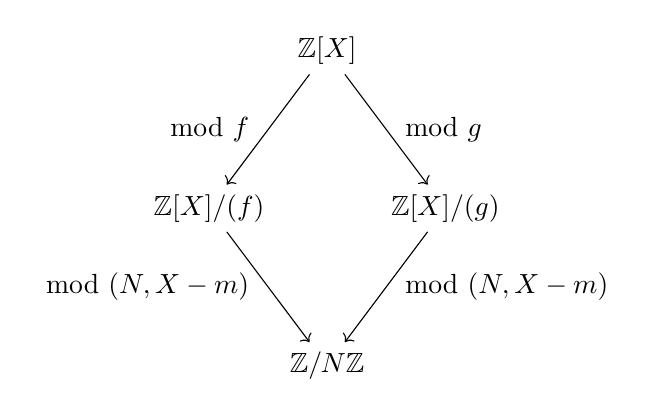
\begin{tikzpicture}
        \node (ZX) at (0, 0) {$\Z[X]$};
        \node (NF1) at (-1.5, -2) {$\Z[X]/(f)$};
        \node (NF2) at (1.5, -2) {$\Z[X]/(g)$};
        \node (ZN) at (0, -4) {$\Z/N\Z$};
        
        \draw [->] (ZX) -- (NF1) node [midway, left] {$\mod f \ $};
        \draw [->] (ZX) -- (NF2) node [midway, right] {$\mod g$};
        \draw [->] (NF1) -- (ZN) node [midway, left] {$\mod (N, X - m) \ $};
        \draw [->] (NF2) -- (ZN) node [midway, right] {$\mod (N, X - m)$};
    \end{tikzpicture}
\end{center}
where $f$, $g$ are coprime, irreducible polynomials with $f(m) = g(m) = 0 \mod N$.
It is common to choose $g = X - m$.
We will work with this simplified situation, so have
\begin{center}
    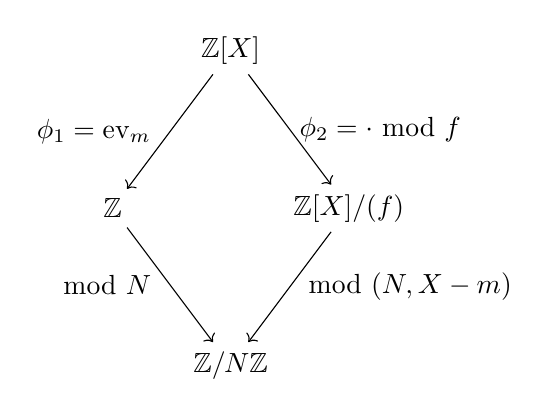
\begin{tikzpicture}
        \node (ZX) at (0, 0) {$\Z[X]$};
        \node (NF1) at (-1.5, -2) {$\Z$};
        \node (NF2) at (1.5, -2) {$\Z[X]/(f)$};
        \node (ZN) at (0, -4) {$\Z/N\Z$};
        
        \draw [->] (ZX) -- (NF1) node [midway, left] {$\phi_1 = \mathrm{ev}_m \ $};
        \draw [->] (ZX) -- (NF2) node [midway, right] {$\phi_2 = \cdot \mod f$};
        \draw [->] (NF1) -- (ZN) node [midway, left] {$\mod N \ $};
        \draw [->] (NF2) -- (ZN) node [midway, right] {$\mod (N, X - m)$};
    \end{tikzpicture}
\end{center}

\section{A special case}
For now assume that $\Z[X]/(f)$ is the ring of integers $\O_K$ in the number field $K = \Q[X]/(f)$, and additionally that it has class number 1 and trivial unit group $\O_K^* = \{ \pm 1 \}$.

We choose a smoothness bound $B$, and have the factor bases $\{ p \in \Z \ | \ \text{$p \leq B$ prime} \}$ in $\Z$ and $\{ \p \leq \O_K \ | \ \text{$\p$ prime ideal over prime $p \leq B$} \}$ in $K$.
Now we search a wide range of values $aX + b \in \Z[X]$ for elements such that both $\phi_1(aX + b) = am + b$ and $\phi_2(aX + b)$ factor over the factor base.

Having found enough, we can multiply a suitable subset and find $aX + b$ such that both
\begin{equation*}
    \phi_1(aX + b) = am + b = x^2 \quad \text{and} \quad \phi_2(aX + b) = y^2
\end{equation*}
are squares.
With some luck now,
\begin{equation*}
    x \mod N \neq \pm y \mod (N, X - N)    
\end{equation*}
and we have found a congruent square.

\section{The general case}
If we use the same approach in the general case, we will end up with $aX + b$ such that
\begin{equation*}
    (\phi_2(aX + b)) = \a^2
\end{equation*}
for an ideal $\a \leq \O_K$.
However, $\a$ might not be principal, and even if $\a = (y)$, we might have that $y \notin \Z[X]/(f)$, or that only $y^2 = \epsilon \phi_2(aX + b)$ with $\epsilon \in \O_K^*$ but $\epsilon \neq 1$.

We fix this by introducing a quadratic character base of characters
\begin{equation*}
    \chi: \Z[X]/(f) \to \{ -1, 0, 1 \}
\end{equation*}
and find $aX + b$ such that not only $(\phi_2(aX + b)) = \a^2$ but also $\chi(\phi_2(aX + b)) = 1$ for all $\chi$ in the character base.
After that, we just hope that these ``problems'' do not occur.

More concretely, we choose another bound $B'$ and take the characters
\begin{equation*}
    \chi: \Z[X]/(f) \to \{ -1, 0, 1 \}, \quad x \mapsto \begin{cases}
        1 & \text{if $x \mod \p$ is a square in $\F_{p^f}$} \\
        0 & \text{if $x \in \p$} \\
        -1 & \text{if $x \mod \p$ not a square in $\F_{p^f}$}
    \end{cases}
\end{equation*}
where $\p$ is a prime ideal of $\O_K$ over the prime number $B < p \leq B'$ and has degree of inertia $f$.
Note that if $p > B$ and $\phi_2(aX + b)$ is $B$-smooth, then this implies that $\chi(\phi_2(aX + b)) \neq 0$.

\section{Choice of parameters}
First of all, we use the following theorem.
\begin{theorem}[Canfield-Erdos-Pomerance]
    Let $n$ be a uniformly random integer $\leq x$.
    Then the probability that $n$ is $B$-smooth is at least
    \begin{equation*}
        \exp( -u \log(u) ) = u^{-u}
    \end{equation*}
    for sufficiently large $x$, where
    \begin{equation*}
        u = \frac {\log(x)} {\log(B)}
    \end{equation*}
\end{theorem}
We ignore the quadratic characters in the following.
Note that for $a, b$ and $\theta := \phi_2(X)$, we know that $\phi_2(aX + b) = a\theta + b$ factors over the algebraic factor base iff $N(a\theta + b)$ is $B$-smooth.
Furthermore
\begin{equation*}
    N(a\theta + b) = a^d \mathrm{MiPo}(\theta)(-b/a) \leq \|\mathrm{MiPo}(\theta)\|_1 \max(|a|^d, |b|^d)
\end{equation*}
In particular, if $|a|, |b| \leq C$ then $N(a\theta + b)$ is of size approximately $mC^d$.

Now we have that both $N(a\theta + b)$ and $am + b$ are $B$-smooth iff $(am + b)N(a\theta + b)$ is.
We assume that this value is uniformly distributed, and of size approximately $m^2C^{d + 1}$.
In other words, for a random $aX + b$ with $|a|, |b| \leq C$, we find a relation with probability
\begin{equation*}
    \exp\left( - \frac {\log(m^2C^{d + 1})} {\log(B)} (\log\log(m^2C^{d + 1}) - \log\log(B)) \right)
\end{equation*}
As we need $B$ such relation to find a solution to the linear equations, we need to search
\begin{equation*}
    \exp\left(\log(B) + \frac {\log(m^2C^{d + 1})} {\log(B)} (\log\log(m^2C^{d + 1}) - \log\log(B))\right)
\end{equation*}
tuples $(a, b)$.
We insert that $\log(m) = \log(N)/d$ and expand, to get
\begin{equation*}
    \exp\left( \log(B) + \frac {\frac 2 d \log(N) + (d + 1)\log(C)} {\log(B)} \left(\log(d) + \log\log(C) - \log\log(B) + O\left(\frac {2\log(N)} {d^2\log(C)} \right) \right) \right)
\end{equation*}
To optimize this, we first consider an approximation of this expression, namely
\begin{equation*}
    \exp\left(\log(B) + \frac {\log(N) + d^2 \log(C)} {d \log(B)} \right)
\end{equation*}
We want to optimize this, subject to
\begin{equation*}
    \exp\left(\log(B) + \frac {\log(N) + d^2 \log(C)} {d \log(B)} \right) \leq \exp(\log(C)) \leq \exp(2\log(C))
\end{equation*}
which just means that there are enough tuples $(a, b)$ with $|a|, |b| \leq C$ to yield the desired amount of relations.

Taking logarithms, we arrive at
\begin{equation*}
    \text{minimize} \quad \underbrace{b + \frac {n + d^2 c} {db}}_{=: R} \quad \text{subject to} \quad b + \frac {n + d^2 c} {db} \leq c
\end{equation*}
We find
\begin{equation*}
    \nabla R = \left(1 - \frac {n + d^2c} {db^2}, \frac d b, \frac {2d^2c - (n + d^2c)} {d^2b} \right)^T
\end{equation*}
This clearly has no optima, so we consider the border of the region, i.e. assume
\begin{equation*}
    c = b + \frac {n + d^2 c} {db} \quad \text{hence} \quad \left(1 - \frac d b\right) c = b + \frac n {db}
\end{equation*}
and we arrive at
\begin{equation*}
    \text{minimize}\quad b + \frac {n(1 - \frac d b) + d^2(b + \frac n {db})} {(1 - \frac d b)db} = b + \frac {ndb - nd^2 + d^3b^2 + nd^2} {d^2b^2 - d^3b} = b + \frac {n + d^2b} {db - d^2}
\end{equation*}
Now we have
\begin{equation*}
    \nabla \left( b + \frac {n + d^2 b} {db - d^2} \right) = \left( \frac {b(b - 2d)d - n} {(b - d)^2d}, \frac {n(2d - b) + b^2d^2} {(b - d)^2d^2} \right)
\end{equation*}
Setting this to 0, and ignoring small constants, we find
\begin{equation*}
    d\log(B)^2 \approx \log(N), \quad d^2\log(B)^2 \approx \log(N)(2d - \log(B))
\end{equation*}
and so $\log(B) \approx \log(N)^{1/3}$ and $d \approx \log(N)^{1/3}$.

\subsection{Details}
To get a more precise estimate without exploding all the expressions, we now use the Landau symbol
\begin{equation*}
    L_N(\alpha, a) = \exp((a + o(1))\log(N)^\alpha\log\log(N)^{1 - \alpha})
\end{equation*}
We set $B = L_N(1/3, b)$ and $C = L_N(\gamma, c)$ and $d = (1 + o(1))\log(N)^{1/3}$.
Then the probability that some tuple gives us a relation (i.e. the images under $\phi_1$, $\phi_2$ are smooth) can now be written as
\begin{align*}
    & \exp\left( - \frac {\log(m^2C^{d + 1})} {\log(B)} (\log\log(m^2C^{d + 1}) - \log\log(B)) \right) \\
    =& \exp\Biggl( -\frac {(2 + o(1))\log(N)^{2/3} + (d + 1)(c + o(1))\log(N)^\gamma\log\log(N)^{1 - \gamma}} {(b + o(1))\log(N)^{1/3}\log\log(N)^{2/3}} \\
    &\Bigl( \log\left((2 + o(1))\log(N)^{2/3} + (1 + o(1))\log(N)^{\gamma + 1/3}\log\log(N)^{1 - \gamma} \right) \\
    &- \log((b + o(1))\log(N)^{1/3}\log\log(N)^{2/3}) \Bigr) \Biggr)
\end{align*}

\printbibliography
\end{document}